\documentclass[12pt]{article}
\setlength{\oddsidemargin}{0in}
\setlength{\evensidemargin}{0in}
\setlength{\textwidth}{6.5in}
\setlength{\parindent}{0in}
\setlength{\parskip}{\baselineskip}
\usepackage{amsmath,amsfonts,amssymb}
\usepackage{graphicx}
\usepackage{array}
\usepackage{fancyhdr}
\usepackage{listings}
\usepackage{flexisym}
\usepackage[table]{xcolor}
\usepackage[utf8]{inputenc}
\graphicspath{ {./images/} }
\pagestyle{fancy}
%Code listing style named "mystyle"
\lstdefinestyle{mystyle}{
  basicstyle=\footnotesize,
  breakatwhitespace=false,
  breaklines=false,
  captionpos=b,
  keepspaces=false,
  numbers=left,
  numbersep=5pt,
  showspaces=false,
  showstringspaces=false,
  showtabs=false,
  tabsize=2
}
%"mystyle" code listing set
\lstset{style=mystyle}
\begin{document}
\lhead{{\bf CSCI 3403 \\ Homework 4} }
\rhead{{\bf Brennon Lee  \\ Fall 2018, CU-Boulder}}
\renewcommand{\headrulewidth}{0.4pt}
\vspace{-3mm}
\begin{enumerate}
% QUESTION 1
\item Students at Some State University (SSU) select very bad passwords. The system administrator decided to use a Bloom Filter to prevent students from using the passwords "cat, dog, fish, and bear". The Bloom Filter uses 3 hash functions (H1, H2, H3) and 10 bits in the hash table. When the hash functions are applied to the prohibited passwords, the results are:

\begin{center}
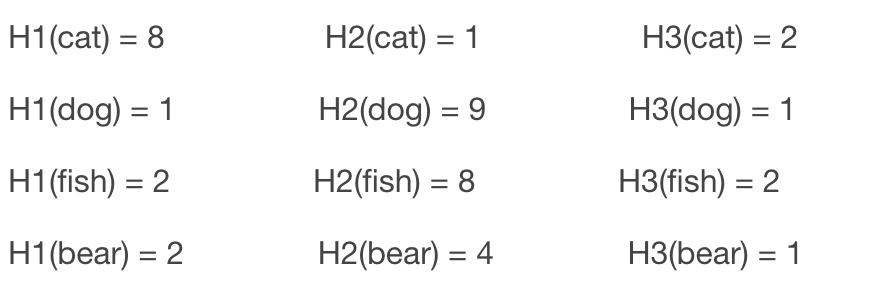
\includegraphics[scale=0.5]{prob1_diagram.png} \\
\end{center}
\begin{enumerate}
  \item Show the resulting Bloom Filter by marking each bit as either 0 or 1. \\
  \begin{center}
    \begin{tabular}{ |c|c|c|c|c|c|c|c|c|c| }
     \hline
     Bit 0 & Bit 1 & Bit 2 & Bit 3 & Bit 4 & Bit 5 & Bit 6 & Bit 7 & Bit 8 & Bit 9 \\
     0 & 1 & 1 & 0 & 1 & 0 & 0 & 0 & 1 & 1 \\
     \hline
   \end{tabular}
 \end{center}

A student selects the password "mouse". Note this is not a prohibited password. Before the password is accepted, it will be checked against the Bloom Filter. Hash functions H1 and H2 are applied to "mouse" and the results are: \\
\vspace{5mm}
H1(mouse) = 4 \hspace{5mm}   H2(mouse) = 8 \hspace{5mm}  H3(mouse) = ?
\item List one value for H3(mouse) that would cause the "mouse" to be rejected as a password or explain why no value of H3(mouse) could cause this. \\

\textbf{One possible value for H3(mouse) is 1. Then because the bits 4, 8, and 1 match the bloom filter bits that are set to one, "mouse" will be incorreclty classified as a member of the set S. Where S is the set of prohibited passwords.} \\

\item List one value for H3(mouse) that would cause the "mouse" to be accepted as a password or explain why no value of H3(mouse) could cause this.

\textbf{One possible value for H3(mouse) is 0. Then because the Bit 0 is not set to 1 on the bloom filter, "mouse" will be valid password.} \\

\end{enumerate}

% QUESTION 2
\item{\textbf{Review Question 3.1}. In general terms, what are four means of authenticating a user's identity?} \\

\textbf{-Something the individual knows: i.e. passwords, PIN, answers to prearranged questions.} \\
\textbf{-Something the individual possesses(token): i.e. Electronic key-cards, smart cards, and physical keys.}\\
\textbf{-Something the individual is (static biometrics): i.e. Fingerprint, retina, face.}\\
\textbf{-Something the individual does (dynamic biometrics): Voice pattern, handwriting, typing rhythm.}\\


% QUESTION 3
\item{\textbf{Review Question 3.8}. Define the terms \textit{false match rate} and \textit{false nonmatch rate}, and explain the use of a threshold in relationship to these two rates.}

\textbf{\textit{False match rate} - Is the percent of invalid inputs which are incorretly accepted.} \\

\textbf{\textit{False nonmatch rate} - Is the percent of valid inputs which are incorrectly rejected.} \\

\textbf{Moving the threshold one way can lead to a decrease in the false match rate but will also increase the false nonmatch rate. And vice versa when moving the other way, decreases the false nonmatch rate and increases the false match rate.}

% QUESTION 4
\item{\textbf{Problem 3.3}. Assume passwords are selected from four-character combinations of 26 alphabetic characters. Assume an adversary is able to attempt passwords at a rate of one per second.}
  \begin{enumerate}
    \item Assuming no feedback to the adversary until each attempt has been completed, what is the expected time to discover the correct password? \\

    \textbf{There are $26^4$ possible passwords and on average an adversary will have to attempt half of them until they guess the correct one.}
    \textbf{So $\frac{26^4}{2}$ words $x$ $1$ guess per second = $228,488$ seconds in total}

    \item Assuming feedback to the adversary flagging an error as each incorrect character is entered, what is the expected time to discover the correct password? \\

    \textbf{There are $26^4$ possible passwords and on average an adversary will have to attempt only half the letters with feedback on each character}
    \textbf{So $26 * 4 = 104$ and on average it will take $\frac{104}{2} = 52$ seconds in total}
  \end{enumerate}

% QUESTION 5
\item{\textbf{Problem 3.4}. Assume source elements of length $k$ are mapped in some uniform fashion into a target elements of length $p$. If each digit can take on one of $r$ values, then the number of source elements is $r^k$ and the number of target elements is the smaller number $r^p$. A particular source element $x_i$ is mapped to a particlar target element $y_j$. }
  \begin{enumerate}
    \item What is the probability that the corret source element can be selected by an adversary on one try? \\

    \textbf{There is a total of $r^k$ source elements so the probability of guessing the correct source element in one try is $\frac{1}{r^k}$} \\

    \item What is the probability that a different source element $x_k (x_i \neq x_k)$ that results in the same target element, $y_j$, could be produced by an adversary? \\

    \textbf{Each target element is mapped by $r^{k-p}$ elements since we are given that $k > p$. There are $r^{k-p}$ target elements. Therefore, there will be $r^{k-p}-1$ unique source elements. Probability that different source element will give the same target element is $\frac{(r^{k-p}-1)}{r^k}$} \\

    \item What is the probability that the correct target element can be produced by an adversary on one try? \\

    \textbf{There is a total of $r^p$ target elements so the probability of guessing the correct target element in one try is $\frac{1}{r^p}$} \\
  \end{enumerate}}

% QUESTION 6
\item{\textbf{Problem 3.6}. Assume passwords are limited to the use of the 95 printable ASCII characters and that all passwords are 10 characters in length. Assume a password cracker with an encryption rate of 6.4 million encryptions per second. How long will it take to test exhaustively all possible passwords on a UNIX system? } \\

\textbf{Total passwords are $95^{10}$ and $\frac{95^{10} passwords}{6.4 * 10^6 passwords/second} = 9.3552647* 10^{12}$ seconds = $296,653$ years}

% QUESTION 7
\item{\textbf{Problem 3.8}. The inclusion of the salt in the UNIX password scheme increases the difficulty of guessing by a factor of 4096. But the salt is stored in plaintext in the same entry as the corresponding ciphertext password. Therefore, those two characters are known to the attacker and need not be guessed. Why is it asserted that the salt increases security?} \\

\textbf{The salt does in fact increase security. If a password is not protected with a salt, an adversary can easily guess the password and once its cracked, they can easily find other users who use the same password (especially if the password list has been stolen). But if protected with a salt, the attacker needs to guess a password $+$ salt for each user. Hence the password file is protected since this is dramatically more diffiuclt.} \\

% QUESTION 8
\item{\textbf{Problem 3.9}. Assuming you have successfully answered the preceding problem and understand the significance of the salt, here is another question. Wouldn't it be possible to thwart completely all passwords crackers by dramatically increasing the salt size to, say, 24 or 48 bits?}

\textbf{Yes, it is possible since the bit increase would make the time amount required to crack the password outside their lifetime.}

\end{enumerate}
\end{document}
